% mycsrf 'for beeing included' snippet template
%
% (c) Karsten Reincke, Frankfurt a.M. 2012, ff.
%
% This text is licensed under the Creative Commons Attribution 3.0 Germany
% License (http://creativecommons.org/licenses/by/3.0/de/): Feel free to share
% (to copy, distribute and transmit) or to remix (to adapt) it, if you respect
% how you must attribute the work in the manner specified by the author(s):
% \newline
% In an internet based reuse please link the reused parts to mycsrf.fodina.de
% and mention the original author Karsten Reincke in a suitable manner. In a
% paper-like reuse please insert a short hint to mycsrf.fodina.de and to the
% original author, Karsten Reincke, into your preface. For normal quotations
% please use the scientific standard to cite

%% use all entries of the bibliography

\subsubsection{Rosegarden ($\bigstar\bigstar\bigstar\bigstar$)}

\parpic(1cm,1cm)[r][t]{
\includegraphics[width=1cm]{logos/rosegarden-300dpi.png}}
\label{Rosegarden}\acc{Rosegarden} versteht sich als Kompositionsumgebung, die
um einen 'MIDI Sequencer' herum aufgebaut worden sei und dabei auch als
Notensatz- und digitales Audiosystem fungiere.\footcite[vgl.][\nopage
wp]{Rosegarden2019a} Als \enquote{MIDI and audio sequencer} und \enquote{musical
notation editor} wolle es \enquote{das Tool der Wahl} für jene sein, die es
vorziehen, mittels Noten zu arbeiten:\footnote{Im Original: \enquote{to serve as
the sequencer of choice for users who prefer to work with music notation}
(\cite[vgl.][\nopage wp]{Rosegarden2019c})}

\begin{quote}\enquote{\textit{Rosegarden allows you to record, arrange, and compose
music, in the shape of traditional score or MIDI data, or of audio files either
imported or recorded from a microphone, guitar or whatever audio source you care
to specify.}}\footcite[vgl.][\nopage wp]{Rosegarden2019c} \end{quote}

Man könne mit \acc{Rosegarden} Musik schreiben, editieren oder komponieren,
diese synthetisieren, mit Effekten anreichern oder abmischen, um sie schließlich
auf CD zu brennen. Und nicht zuletzt biete \acc{Rosegarden} eben den
\enquote{[\ldots] well-rounded notation editing support for high quality printed
output via LilyPond}.\footcite[vgl.][\nopage wp]{Rosegarden2019c}

Stellt man dem die These zur Seite, dass der \enquote{Kern eines Sequenzers
[\ldots] die Speicherung und Über\-mitt\-lung einer Partitur an einen
Tonerzeuger (sei)}, die \enquote{ [\ldots] in einem maschinenlesbaren Format
(vorliege)}, und dass diese Partitur \enquote{[\ldots] Tonhöhe, Tondauer und
ggf. weitere Aspekte der wiederzugebenden Noten einer oder mehrerer Stimmen in
ihrer zeitlichen Reihenfolge an ein Gerät (weitergäbe), das entsprechende Töne
(erzeuge)}\footcite[vgl.][\nopage wp]{WpedSequencer2018a}, dann gewinnt man
damit eine recht genaue Vorstellung von dem, was \acc{Rosegarden} leisten will:
Es erlaubt den Import von \acc{MIDI}-Aufnahmen, bietet die Möglichkeit, diese zu
korrigieren, zu modifizieren, zu arrangieren und wieder
abzuspielen\footcite[vgl.][\nopage wp]{Rosegarden2019c}. Ein Seiteneffekt des
Angebots ist, dass diese Modifikationen auch visuell über einen Noteneditor
erfolgen können.\footcite[vgl.][\nopage wp]{Rosegarden2019d}

Als Open-Source-Software wird der Quelltext von \acc{Rosegarden} öffentlicht
gehostet und weiterentwickelt.\footnote{\cite[vgl.][\nopage
wp]{Rosegarden2019e}. Die Projektseite gibt an, das Programm werde unter der
GPL-2.0 Lizenz distribuiert. Damit ist \acc{LilyPond} freie Software.} Die
Dokumentation wird als Wiki gepflegt\footcite[vgl.][\nopage wp]{Rosegarden2019c}
und auch in thematischen Teilenbereichen bereitgestellt\footcite[vgl.][\nopage
wp]{Rosegarden2019d}. Daneben gibt es noch spezielle
Tutorials\footcite[vgl.][\nopage wp]{Rosegarden2019b}, die ausgehend von einem
bestimmten Aspekt in die Nutzung von \acc{Rosegarden}
einführen.\footcite[vgl.][\nopage wp]{McIntyre2008a}

Vom Format her erlaubt es \acc{Rosegarden}, außer dem eigenen Dateityp auch
\acc{MIDI}- und \acc{MusicXML}-Dateien zu öffnen bzw. zu importieren. Beim Export
wird u.a. noch das \acc{LilyPond}-Format angeboten. Startet man einen
\acc{MIDI}-Server -- etwa \acc{timidity}\footnote{über eine Shell per
\texttt{timidity -iA}} --, bevor man \acc{Rosegarden} aufruft, können die
geladenen Noten außerdem erfolgreich abgespielt werden.

Unsere Referenzkadenz II vermag \acc{Rosegarden} problemlos als MusicXML-Datei
zu lesen, sofern diese keinen Text, also keine Harmonierungssymbole enhält.
Selektiert man beide Tracks und ruft über das Menue die Notenvisualierung
auf\footnote{\texttt{Select/Edit With/Open in Notation Editor}}, wird der
Notentext auf dem Bildschirm angezeigt:

\begin{center}
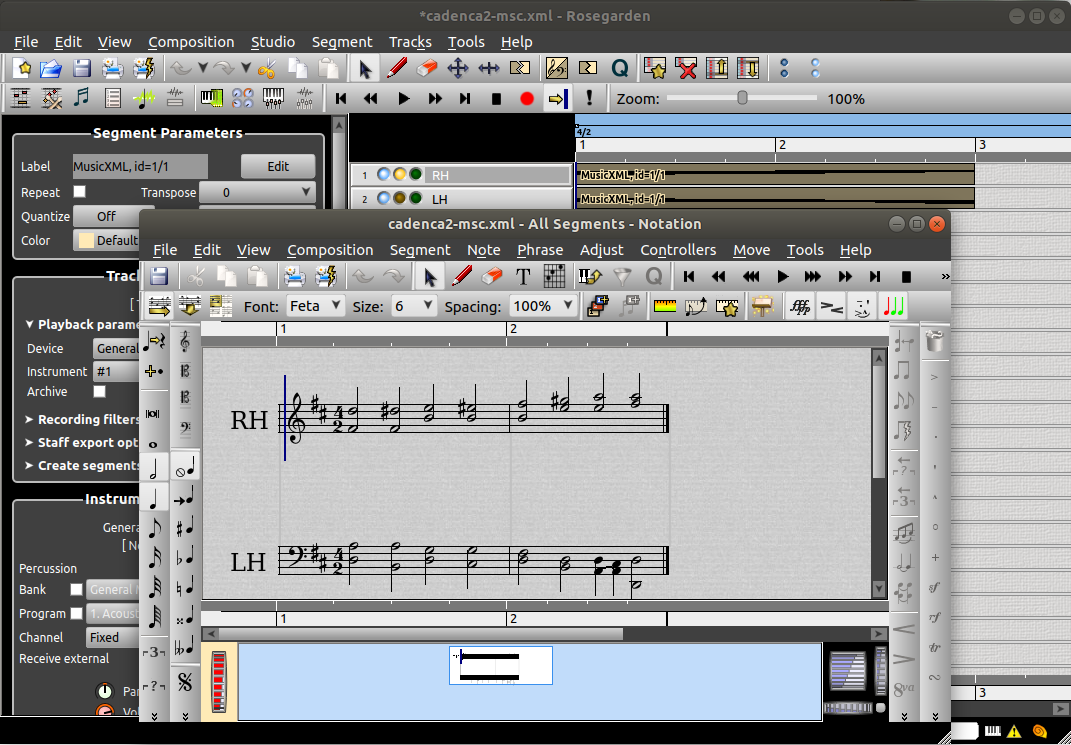
\includegraphics[width=0.9\textwidth]{frontends/rosegarden/rosegarden-cadenca2-300dpi.png}
\end{center}

Das Editieren des Notentextes ist gewöhnungsbedürftig, aber nicht unmöglich.
\acc{LilyPond}-Code kann nicht direkt eingegeben werden. Damit steht unsere
kleine Zusatzbibliothek für die Harmonieanalyse nicht zu Verfügung, allenfalls
die Umfunktionierung die normalen Liedtextfunktionalität. Wenn man unsere
Referenzkadenz als \acc{LiyPond}-Code exportiert, kann man das Ergebnis ohne
Abstriche z.B. in \acc{Frescobaldi} wieder einlesen.

Für die Musikwissenschaftler, die ihre Beispiele eher über \acc{MIDI}-Kanäle
eingeben wollen, ist Rosegarden sicher ein geeignetes Frontend und verdient vier Sterne.


% this is only inserted to eject fault messages in texlipse
%\bibliography{../bib/literature}
